\chapter[Conclusion]{Conclusion}\label{c:conclusion}

The core aim of this thesis was to examine how to enable co-creativity between humans and generative artificial intelligence. Specifically, the following core research question was posed. 

\begin{quote}
\textbf{Core Research Questions:}
\emph{How can we design generative AI systems that act as effective co-creators, maintaining human agency while effectively leveraging the creative potential of this technology?}
\end{quote}

Broken down into the following sub-questions: 

\begin{quote}
\textbf{Sub-Questions:}
\begin{enumerate}
    \item \emph{Which interaction design principles can guide the development of effective co-creative systems?}
    \item \emph{What is the potential of modelling dialogue in interaction design to enable effective human--AI co-creativity?}
    \item \emph{How does interaction design influence the role that humans and AI play in creative production?}
\end{enumerate}
\end{quote}


I examined these questions through a mixed-methodology approach, developing and testing prototypes with users from a design research perspective, and engaging in creative practice through collaborations with teams working on real-world creative productions.

In the following sections, I will first articulate the core argument, which is the answer to the research questions above. 

After than, I will elaborate further on each question. I will do so in reverse order. First discussing how interaction design influences the roles of humans and AI in creative activities, and the influence of this in the effectiveness of the interaction and the agency of the human. 

Then I will discuss the value of modelling in interaction design to enhanc interaction. 

And finally, I will provide a set of design principles. 

\section{Core argument}

% Put a brief introduction one or two sentences as preambles sentence here.

%% Leave mostly unchanged, this is the core argument
Interaction with generative AI in creative activities often diminishes user creative agency through what I term severed agency: a disconnect between intention and action. 

This severing emerges from a shift in role distribution. Humans increasingly operate within the intentional space, where creative goals, visions, and high-level decisions reside, while AI systems take on roles in the action space, where concrete artefact-level operations such as drawing, writing words, or playing notes occur. 

This ultimately leads to less effective interactions, where users struggle to translate intention into outputs, and where instead of co-creativity, client-producer relationships of creative automation emerge.

Dialogic design is a promising approach to increase human agency and the effectiveness human-AI co-creativity through more closely aligning intention and action in human-AI interaction. Dialogic design involves creating context-aware iterative interactions that promote mutual adaptation and understanding. In such systems, humans and AI engage in bidirectional communication not only through language but through the creative artefact itself. 

In the last section, as the core contribution of this thesis, I articulate a set of design principles that operationalise dialogic design, offering concrete guidance for the development of co-creative AI systems.


\section{Research question 1: how interaction design influences roles assumed by humans and AI, and the consequences on effectiveness and agency}


- We can understand creativity as consisting of moving between two spaces consisting of two spaces: the intention space and the action space.

- In the intentional space, are goals, taste, decisions, directions, intention to express. 

- In the action space, are writing words, playing notes, or drawing lines. Doing actions at the artefact level. 

- This distinction is found across the literature \cite{Palani2024-on}
- And I argue it is core to understand the shifting of roles between humans and ai in creative activities
% here add other references that may be worth considering, add a comment for me to search it, that talk about a distinction between an intentional and execution space.

\begin{figure}
    \centering
    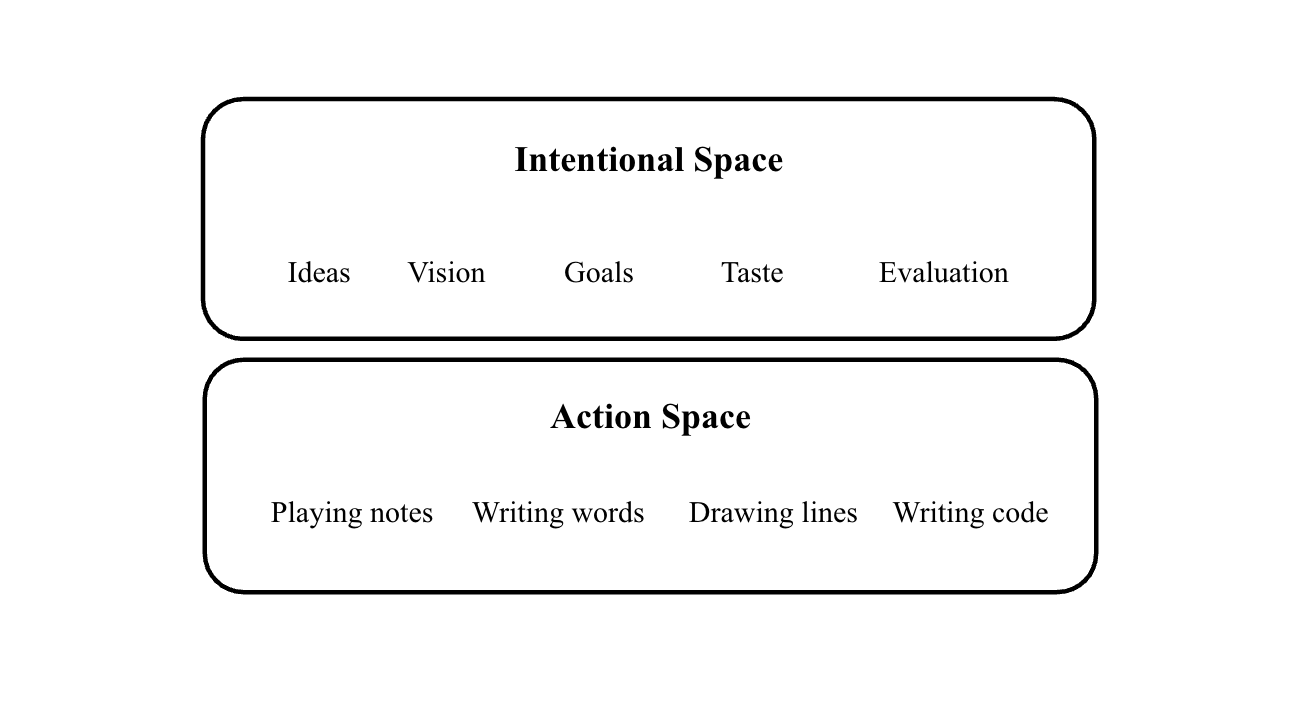
\includegraphics[width=1\linewidth]{intention action spaces.png}
    \caption{Intention and action space}
    \label{fig:enter-label}
\end{figure}

- The research in this thesis
- And emerging literature shows that
- When interacting with AI
- Humans largely assume roles in the intentional space
- And AI assumes roles at the intentional space

- In Chapter 4, I discussed how humans tend to assume those roles. 
- When discussing the roles assumed: participants often that: 

"I was the curator of the story—I picked the pieces I liked and left the rest." 

"I gave it the idea, and it just took it from there, writing almost everything."

"I gave it the skeleton of the story, and Vorges fleshed it out—almost like giving the recipe and having it
cook the dish." (Participant 11, Chat-only)

"I asked it to write a paragraph about a dystopian future, and it did everything from there." (Participant
6, Chat-only

"I started with a basic introduction, and Vorges expanded it into a complete narrative." (Participant 3,
Chat-only)

"Vorges wrote 90\% of the story based on my prompts. I just tweaked it a bit."


- People tended to describe their roles specifically as director, editor, curator.

- This echoes similar findings in the literature

- In an extensive review of the emerging roles and workflows that humans and AI assume in creative workflows

- Palani et al \cite{Palani2024-on} found users are increasingly assuming assume roles at the "Project" level while AI assumed roles at the "Artifact" level

- This also aligns with practice. The newly coined term vibe-coding
- Was described by AI researcher Andrej Karpathy as prompting the AI to write code, barely being involved in reading it or understanding it, and mostly forgetting the code even exists

- \begin{quote}
"[I] forget that the code even exists. [...] I barely even touch the keyboard. I ask for the dumbest things like "decrease the padding on the sidebar by half" because I'm too lazy to find it. I "Accept All" always, I don't read the diffs anymore. When I get error messages I just copy paste them in with no comment, usually that fixes it. The code grows beyond my usual comprehension [...] It's not too bad for throwaway weekend projects, but still quite amusing. I'm building a project or webapp, but it's not really coding"
\end{quote}

Weisz argues: "Generative AI technologies have introduced a new paradigm of human-computer interaction, what Nielsen refers to as “intent-based outcome specification” [127]. In this paradigm, users specify what they want, often using natural language, but not how it should be produced."

- This begins to highlight that this shifting of roles, where humans move into the intentional space and AI assumed mostly roles at the intentional space, introduces a fundamental tension: a disconnect between intention and action.

- If we accept the standard definition of agency as intentional action, it's clear how this may affect human creative agency, especially given the difficulty to steer models, to succesfully get them to do what we want, and to understand how and why they are doing it. 

- I propose a term for this: severed agency. 

- Let's discuss this further


\begin{figure}
    \centering
    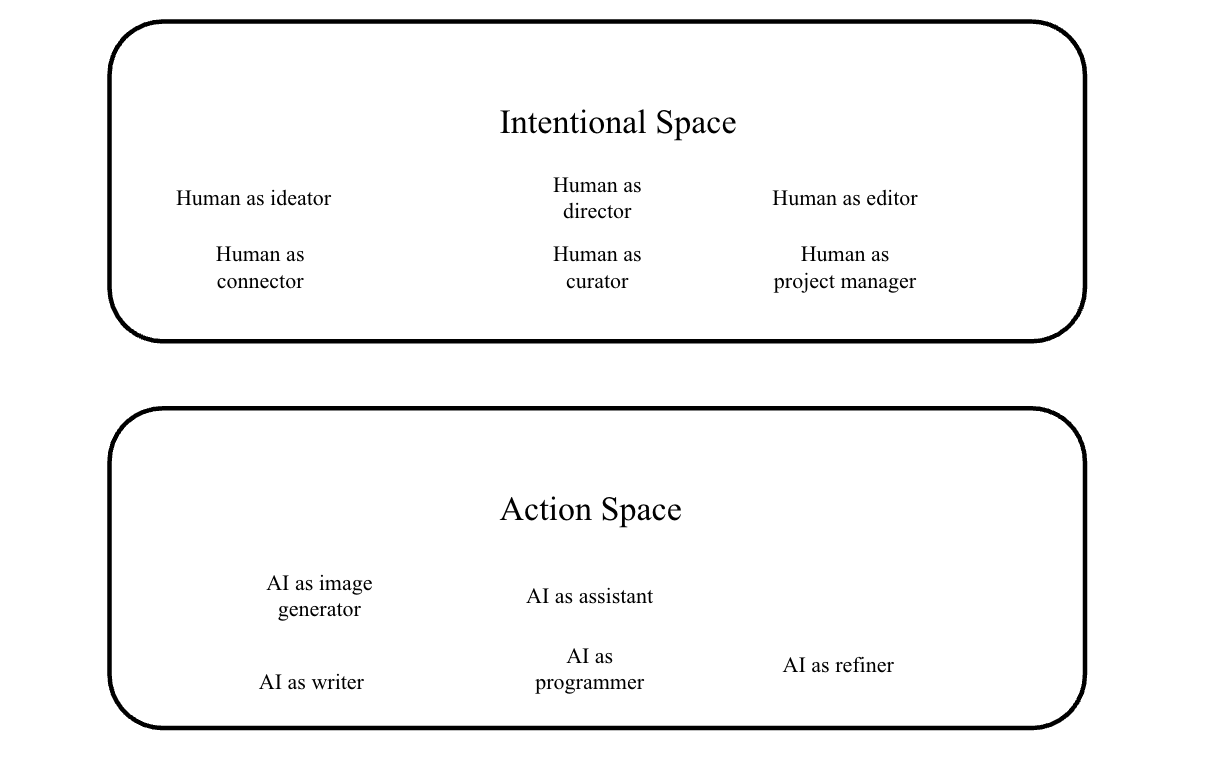
\includegraphics[width=0.75\linewidth]{rolesinspaces.png}
    \caption{Enter Caption}
    \label{fig:enter-label}
\end{figure}

\section{Severed agency}

- Let's discuss further the effect of this separation between intentional and action spaces

- And how this leads to severed agency

- And affects the effectiveness of human-AI interaction and co-creativity

\subsection{Failing to align instructions to outputs}

- First, as we discussed above, agency can be understood as intentional action

- Failing to align intention and action by definition reduces agency. 

- Severed agency occures through three mechanisms:

- On a first level, agency is diminished simply by the process of a tool failing to produce what the user expects. 

For example, in my case study with the AFR in chaper 6, I identified the main limitations in our creative process to use generative AI image models was controlling their outputs, both stylistically and structurally, achieving consistent results across iterations that allowed us to refine images towards cnvergence.  

Similarly, Palani et al, in the same study discussed beore how humans tend to assume more Project Level roles while AI assumed more artifact level roles. They also found that two of the main limitations for adoption of AI in creative activities are: "Aligning and Assessing Stochastic Model Outputs With Intent." and "Articulating creative goals"

- For example: one participant claimed: "I was prescriptive in my prompt, and I thought I nailed it. But the model never did, and it still doesn’t. That drives me crazy and keeps me surprised, delighted, and sometimes annoyed."

Another user describes: "at times, I didn’t have the vocabulary to ask the model to help me. I think your background knowledge matters: someone with an art history background knows how to prompt a specific style, unlike someone who doesn’t." Furthermore, it is hard to articulate tacit knowledge such as style and expertise."

- This a notable feature of generative AI systems

- Weisz \cite{Weisz2024-io} terms this as "generative variability"
- Where often users dont know what they will get. This can be a feature. As the participant cited above described: this can introduce surprise and delight. But in serious creative production, this can lead to annoyance, and simply unasble tools. 

Weisz argues: "With generative AI applications, users will need to develop a new set of skills to work with (not against) generative variability by learning how to create specifcations that result in artifacts that match their desired intent."

But this is notably hard. 

- Much literature has discussed their black box nature, which involves issues of explainability \cite{Linardatos2020-uq} both at the alrogithmic and interaction design level \cite{, Llano2022-tiEl-Assady2022-qc, Zhu2018-zd}.

- It is not only an issue to prompt adherence: it is one of different preferences. What a user considers "a beautiful image of a flower" will differ between users. 

- So on a first level, erosion of agency and effectiveness of interaction and misalignment between intention and action, stems largely from a lack of mutual understanding between human and AI: the human cannot understand how inputs map to outputs. The system is simply too opaque and variable to generate such mappings, particularly in prompt-only interaces. 

And second, we can understand models not understanding users: they are trained to fulill user requests, yet are not able to infer what a user truly wants when describing something with a particular word. 

Here begins to emerge the value o interaction that helps align tis understnding. By helping the user form mental models o the system, enabling dialogue to align meaning, and enabling users to participate at the action level to provide examples and guide the creative artifact. I will discuss this further in the section on dialogue. 

\begin{figure}
    \centering
    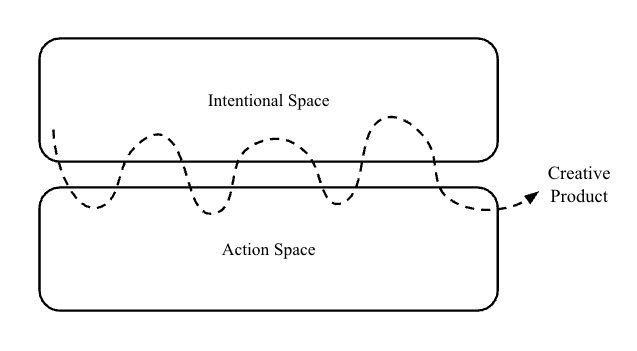
\includegraphics[width=1\linewidth]{alignedintention.png}
    \caption{Aligned intention and action}
    \label{fig:enter-label}
\end{figure}

\subsubsection{Erosion of skills}

On a second level, agency is affected in the longer term, through the process of erosion of skills.

A growing literature finds that overreliance on AI to execute tasks on behalf of users can lead to critical skill loss \cite{Heersmink2024-mk}, losing o critical skills \cite{Rafner2021-tm}.  


Gerlich found that overreliance of AI to perform writing tasks is linked to loss of criticial thinking skills  \cite{Gerlich2025-as}. In recent study by Lee et al published at the Conference on Human Factors in Computing Systems 2025 (CHI) \cite{Lee2025-dw} found that use of generative in knowledge workers AI was linked to less congitive effort, and reduced self-confidence. While not specific to a creative scenario, this paper highlights a potential impact on creative agency. Self-confidence in one's ability to be creative and complete a creative task has been found to be crucial in creativity, is termed creative self efficacy, and it is found to be one of the main determinants of creative achievement. 

However, research also shows this is largely mediated by the level of involvement of the user at the artifact level. For example, a study by \cite{Kim2023-wt} found that a generative writing tool that was repurposed to act as a Socratic tutor, asking questions to the student instead of merely writing based on their request, was able to increase their writing skills. 

Similarly, a study by \cite{Essel2024-qc} found that using an LLM helped increase students criticial and reflective skills when they were provided with a set of prewritten prompts to use with the model to stimulate critical thinking. Increasingly, providing prompts and prompt structures can be understood as interaction design with generative AI. 

A study by \cite{Jia2024-vp} "exploring when and how artificial intelligence augments employee creativity" in the context of sales found when AI was used to automate lead generation, prescreening clients, so that employees could focus on persuasion of high potential clients, employees showed greater creativity in answering and persuading customers. Arguably this is a result of designing a system that focused on automating a tedious, low-skilled task, so that employees could focus energy on exercising their core sales skills. Interestingly, authors also show that this effect was more pronounced on already highly skilled workers. This study highlights a prime example of the automation-augmentation paradox: while often the theoretical stance is to favour augmentation over automation, \cite{Raisch2021-nw} argue these cannot be neatly separated. In this case, the automation of this specific task lead to employee creative augmentation, highlighting the need to clearly define which is the most valuable task to automate to let human skills be exercised, and design systems accordingly.  

\section{Erosion of enjoyment and involvement}

The third way in which humans shiting to roles in intentional space and AI shifting to roles in the executive space is in the erosion o one of the core features of creativity: intrinsic enoyment. 

Take for example, the case of a participant in my Chapter 4, who described their experience using the Vorges tool to write:

 "[it] made me feel like I was cheating somehow. It does not feel like my work, even though I gave all the ideas. Also, I believe there is satisfaction in putting a lot of effort/dedication/patience into something. Vorges made everything so simple, fast, and easy that it felt artificial and no real satisfaction came as a result." 

A similar sentiment is echoed by famed artist and one of the pioneers of (pre-AI) generative art Brian Eno : 

"In my own experience as an artist, experimenting with AI has mixed results. I’ve used several “songwriting” AIs and similar “picture-making” AIs. I’m intrigued and bored at the same time: I find it quickly becomes quite tedious. I have a sort of inner dissatisfaction when I play with it, a little like the feeling I get from eating a lot of confectionery when I’m hungry. I suspect this is because the joy of art isn’t only the pleasure of an end result but also the experience of going through the process of having made it. When you go out for a walk it isn’t just (or even primarily) for the pleasure of reaching a destination, but for the process of doing the walking."
\cite{Eno2024-rj}

Compare this with a user in a second experiment in my chapter 4, using a prototype that afforded contributing at the action level, using a shared editor alongside a chat. 

P4 Common AI: "I really-really enjoyed writing this. I even had a deep moment of reflection, my writing was nostalgic and sad, but I was able to use AI to steer it in the right direction, it gave me confidence that I was also writing with correct grammar and spelling, English is not my first language and while I am proficient, I can still use proofreading to ensure good quality, this tool helped me with it."


P9 shared: “I liked how my original ideas were still retained, and AI was used to complement my intentions. It forced
me to put in some effort and do the majority of the work.”

P22 emphasized: “It adds an element of working together, which I think is the moral problem with current AI tools—they
often seem like they’re doing all the work.”

- In sum, humans assuming roles at the intetional space reduces agency and co-creative effectiveness by reducing eroding involvement and intrinsic enjoyment in the activity itself. 
- Focused on the output rather than the process
- Intrinsic motivation is a crucial aspect of creativity
- People largely create for the sake of it, and generally do it better when they enjoy it \cite{Amabile1996-pt, Csikszentmihalyi1997-ui}
- As such, enjoyment has been a crucial dimension of analysis and design for co-creative systems \cite{Davis2016-te, Cherry2014-ty, Rezwana2022-ui, Clark2018-yf, Lawton2023-gd, Yuan2022-kb, Li2024-yh, Kantosalo2015-pk, Resnick2005-fs}
- Paradoxically, generative AI may lead to co-creative systems that are less enjoyable and with that hinder effectivness and agency

%% Brief very concise wrap up here
I outlined how separation between intention and action can lead to reduce user agency and reduced effectiveness of interaction with AI in creative activities

In the following section I will address in more detail specific ways in which interaction design can address these challenges. 
More specifically, I will discuss how dialogic interaction can contribute to this

\section{R3: What is the potential of modelling dialogue in interaction design to enable effective human-AI co-creativity?}


- In chapter 3, I defined dialogue as a mechanism to form mutual understanding.
- Dialogue involves a process of agreeing, clarifying, refining or elaborating upon concepts, representations, goals, plans or roles among a number of actors
- Applied to human-AI co-creativity, dialogic interaction involves a design patterns aligning meaning to create something. 
- This where its value resides: enabling better alignment between intention and action

- Its important to clarify that while dialogue may be associated simply with conversational interfaces
- How I define dialogue here involves more than that
- As I defined in my own terms as working definitions throughout this thesis

- Conversational interaction simply involves verbal exchanges, through text or voice
On the other hand, I proposed dialogic interaction can be understood as a richer process focused on aligning meaning, through mutual understanding and influence
- This happens partly, but noy only, through bidirectonal communication, chats or else. 
- But it may also happen through contributions to an evolving product itself
- But as musicians can be understood to be having a creative dialogue
- Or how a creator can have a dialogue with a material, in a back and forth iterative loop of mutual adaptation

- These ideas are not new to this thesis. 
- In fact, proposing that humans engage with dialogue with machines is common in human computer interaction \cite{Suchman2006-bs}. 
- In a paper discussing "what is interaction" Hornbaek and Oulasvirta \cite{Hornbaek2017-wg} drawing from relevant HCI work, proposed it is common in the literature to simply see interaction between human and computer can be simply seen as a dialogue. as a cycle of communication acts channeled through input/output from the machine perspective, or perception/action from the human perspective
- Norman’s stages go from users formulating their goal, over specifying and executing the actions needed to move that goal forward, to perceiving the resulting system state and relating that to the goal. Understanding interaction-as-dialogue stresses the need for users’ acts to be understood by the computer and for users to understand the computer. 
- Thus mutual interaction
For Norman, this means that \textbf{mapping} and \textbf{feedback} become crucial concepts for appreciating user interfaces. Mapping requires the user to figure out how to achieve an intention with an interface or the task where “the user must translate the psychological goals and intentions into the desired system state, then determine what settings of the control mechanisms will yield that state, and then determine what physical manipulations of the mechanism are required”
- \cite{Hornbaek2017-wg} Hornbaek argues these in turn are related to the concepts of gulf-of-execution and gulf-of-evaluation, which describe breakdowns when users seek to express their intentions and interpret feedback from the system.

- Similarly, arliest discussions on human-AI co-creativity and mixed interaction, such as Allen's seminal paper on Mixed-Initiative Interaction, explicitely stated it was based on the properties of human dialogue. 
- He proposed that: "While natural-language interaction is the typical form of human dialogue, dialogue models can be characterized in terms of any communication protocol and are independent of natural language. People even engage in dialogues in other modalities, using gestures, drawing, and the like. A computer offers yet further modes of communication, graphics-based user interfaces, menu-base systems, and so on, used both for system output and point-and-click input. By dialogue, I refer to specific mechanisms such as contextual interpretation, turn taking, and grounding, that would be needed with any communication modality.

While Yannakakis \cite{Yannakakis2014-zs} developed a framework for mixed-initiaitive co-creativity, and Muller et al \cite{Muller2020-nv} developed a framework for mixed-initiative generative AI interfaces, no further work developed the concept of dialogic interaction. 

So in chapter 3, I aimed to take dialogic seriously as an interaction design concept drawing from the literature on dialogue, HCI to contruct a first conceptualisation of dialogue as containng the following key elements: 

- Iteration
- Bidirectional communication
- Mutual understanding 
- Mutual influence 
- Shared space for creation 
- Context awareness 

With this, I will now go back to my research and discuss how these elements influence agency and effectiveness of co-creativity
And how each can be operaitonalised in design principles. 

They are closely interrelated, aspects of one affect others. 

\subsection{Iteration}

- Let's begin with the context of iteration. 
\begin{itemize}
    \item Iteration in creative activities is crucial, and it involves \textbf{guided exploration} of different alternatives and further pursuit of them \textbf{through refinement.} 
    \item However, it is notably hard with generative AI systems
\end{itemize}
- As discussed in the chapter 6 study AFR case study in chapter 6.
- As I discussed iteration was one of the main challenges we faced in the process. 
- Generating an image we liked, and pursue this stylistic direction
- However, systems due to their generative variability 
- indeed \cite{Park2024-gw} in a A Thematic
Analysis of How Professional Designers Use Generative AI Image Generation Tools, found one of the key limitations is "the lack of support for the iterative nature of design processes in GenAI tools". 

- But this process, as Norman notes, also serves to help the user build mental maps of the system
- Iteration is needed to help users map inputs to outputs, and help close the gap between intention and action

- Now iterative refinement of outputs, is both a technical and interaction problems
- Currently, new models with varying levels of success afford users to make edits, such as Flux Kontext and gpt-image-1 iteratively
- This was not possible at the time of my case studies


- However, even in the absence of such capabilities, interaction design can still afford iteration

- To provide an example, in the same case study, I logged in a document different experiments, varying a few parameters and prompt at a time, and logging the resulting image, in order to undertand how inpus mapped to outputs



\begin{figure}
    \centering
    
\includegraphics[width=0.5\linewidth]{albo2.png}
    \caption{Enter Caption}
    \label{fig:enter-label}
\end{figure}

\begin{figure}
    \centering
    
\includegraphics[width=0.5\linewidth]{albo.png}
    \caption{Albo1}
    \label{fig:enter-label}
\end{figure}

\begin{figure}
    \centering
    
\includegraphics[width=0.5\linewidth]{albosmiling.png}
    \caption{Enter Caption}
    \label{fig:enter-label}
\end{figure}




- Similar prompting practices have emerged, where practitioners log results based on different settings

- This represents a cleaer opportunity for interaction design
- Tools today mostly lack support for this

- One could imagine a tree like interface that allows users to explore different avenues
- Allowing them to backtrack and building rich histories
- Which would align with principles of tools to support creative thinking  \cite{Resnick2005-fs}

- Another alternative is interactions and tools that afford feeding outputs back as inputs

- Another alternative is remixing and recombination of outputs
\begin{itemize}
    \item In a study with design \cite{Zhou2024-vp} compared linear vs nin-linear dynamics o co-creation. 
    \item Finding iterative interaction better supported converging towards a goal. 
    \item They enabled this iteration through “iterative remixing” where users could combine elements of previous generations. 
\end{itemize}

- Another option is exploratory interfaces that suport semantic navigation in a space
- Schaerf \cite{Schaerf2024-gf} argues latent spaces can be seen as multidimensional spaces of potentiality
- Indeed generative systems build latent spaces that invite rich exploration
- And more explicit implementation of the metaphor of creativity as an exploration of a space of possibilities \cite{Boden2003-hk, Wiggins2019-yj}
- For example, 2D interfaces where users move up or down in directions that are mapped to outut charateristics. 
- For example, Davis showed an interface that enabled exploration of a visual space better afforded ideation in a design setting than text to image interfaces \cite{Davis2024-ml}

\begin{figure}
    \centering
    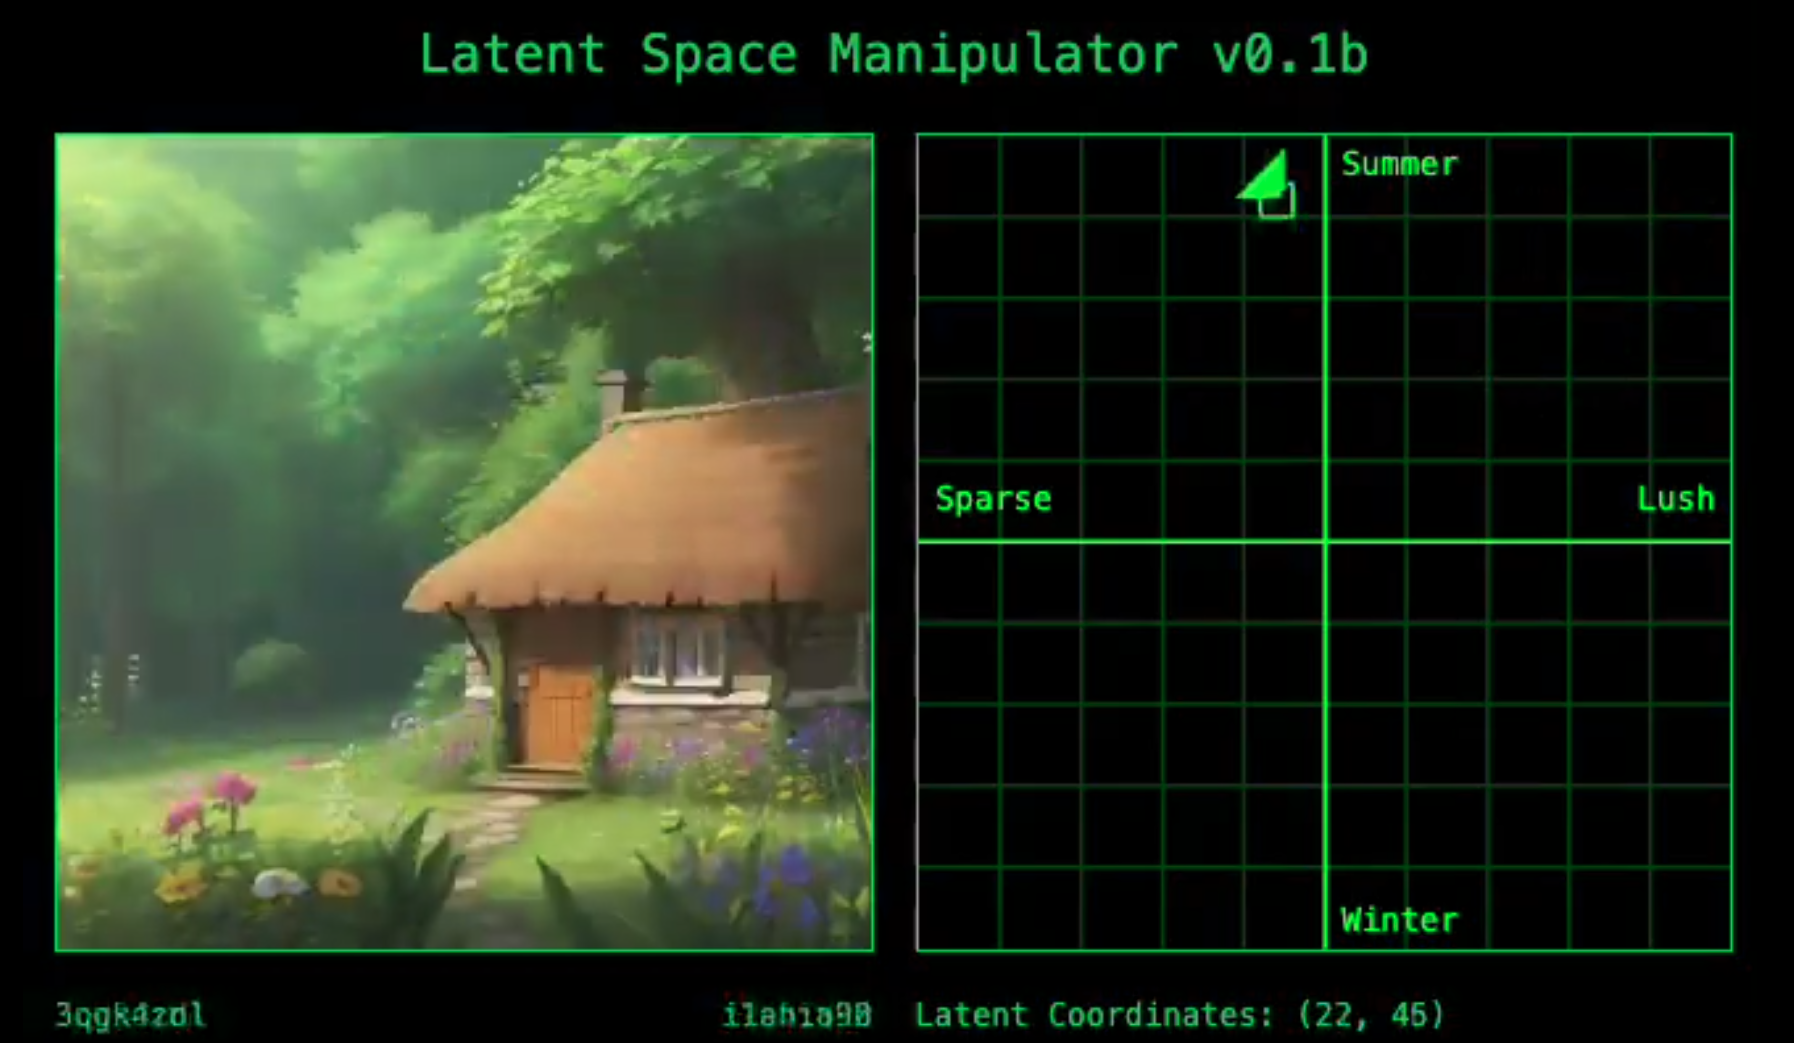
\includegraphics[width=1\linewidth]{latentspacemanip.png}
    \caption{Prototype by Michael Feldstein}
    \label{fig:enter-label}
\end{figure}


\begin{figure}
    \centering
    
\includegraphics[width=1\linewidth]{image.png}
    \caption{Mario Klingeman}
    \label{fig:enter-label}
\end{figure}

\begin{figure}
    \centering
    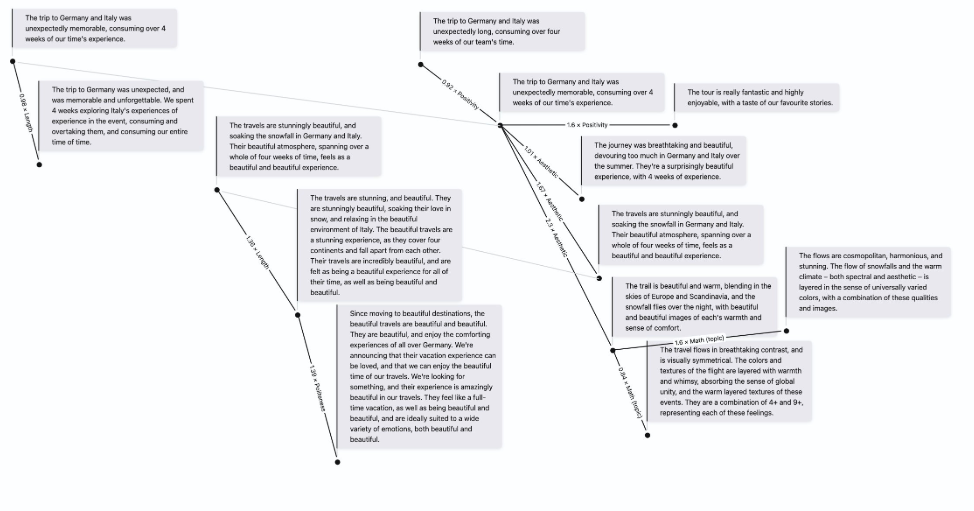
\includegraphics[width=1\linewidth]{linus.png}
    \caption{Linus Lee}
    \label{fig:enter-label}
\end{figure}

\begin{figure}
    \centering
    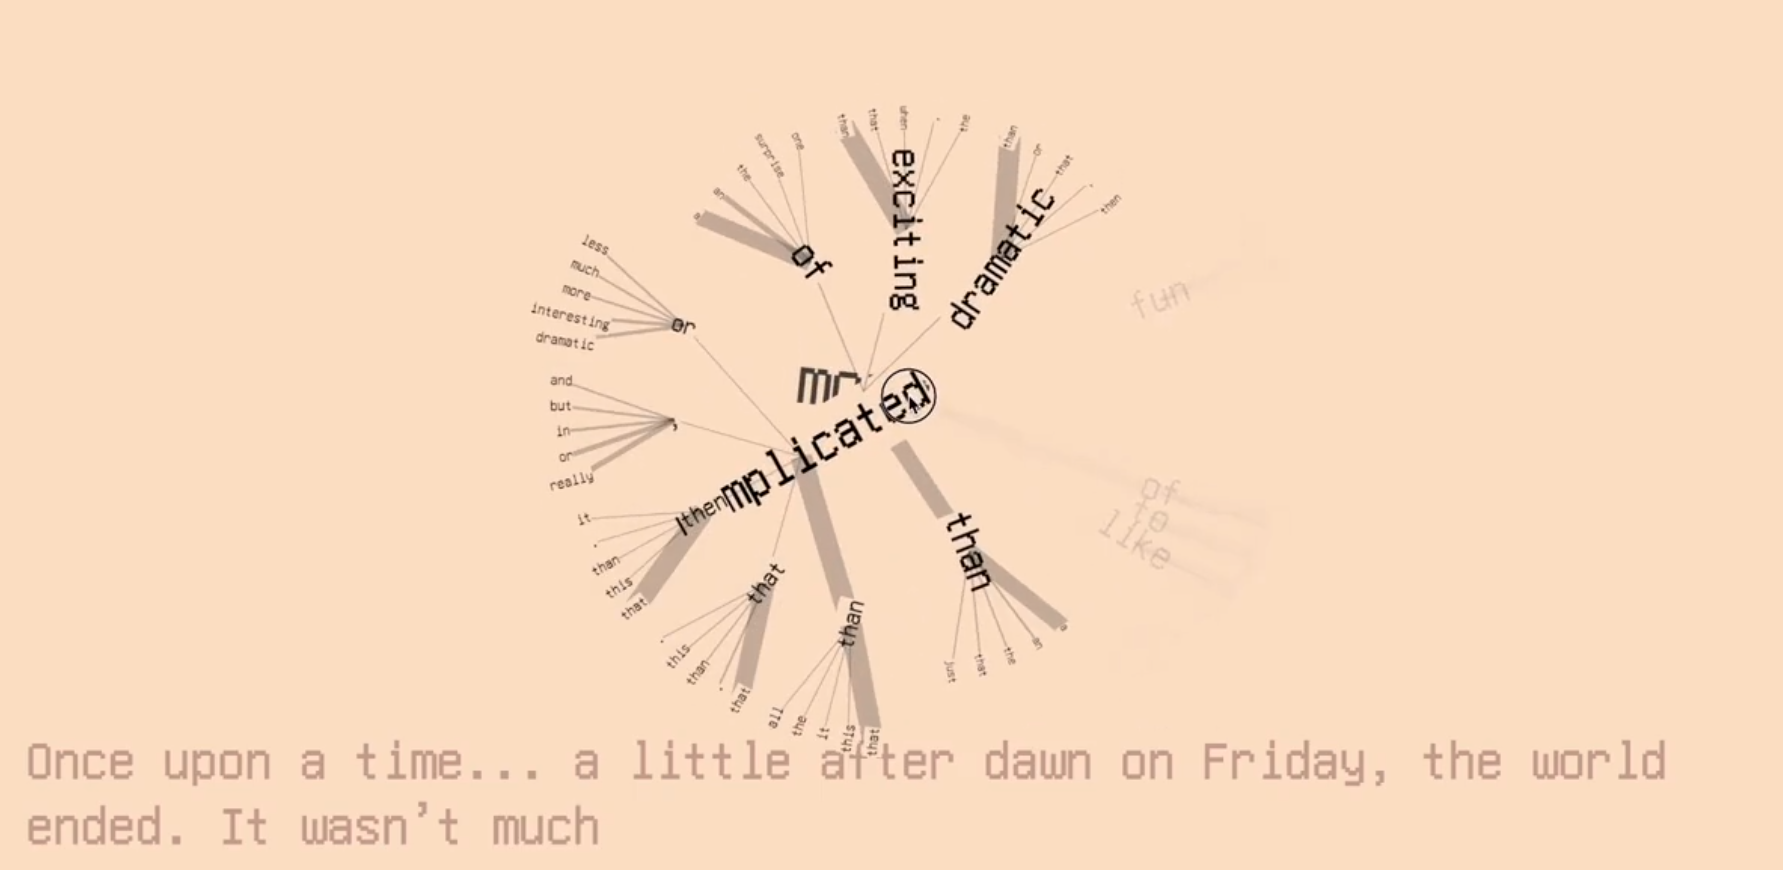
\includegraphics[width=1\linewidth]{treewords.png}
    \caption{Enter Caption}
    \label{fig:enter-label}
\end{figure}

\begin{figure}
    \centering
    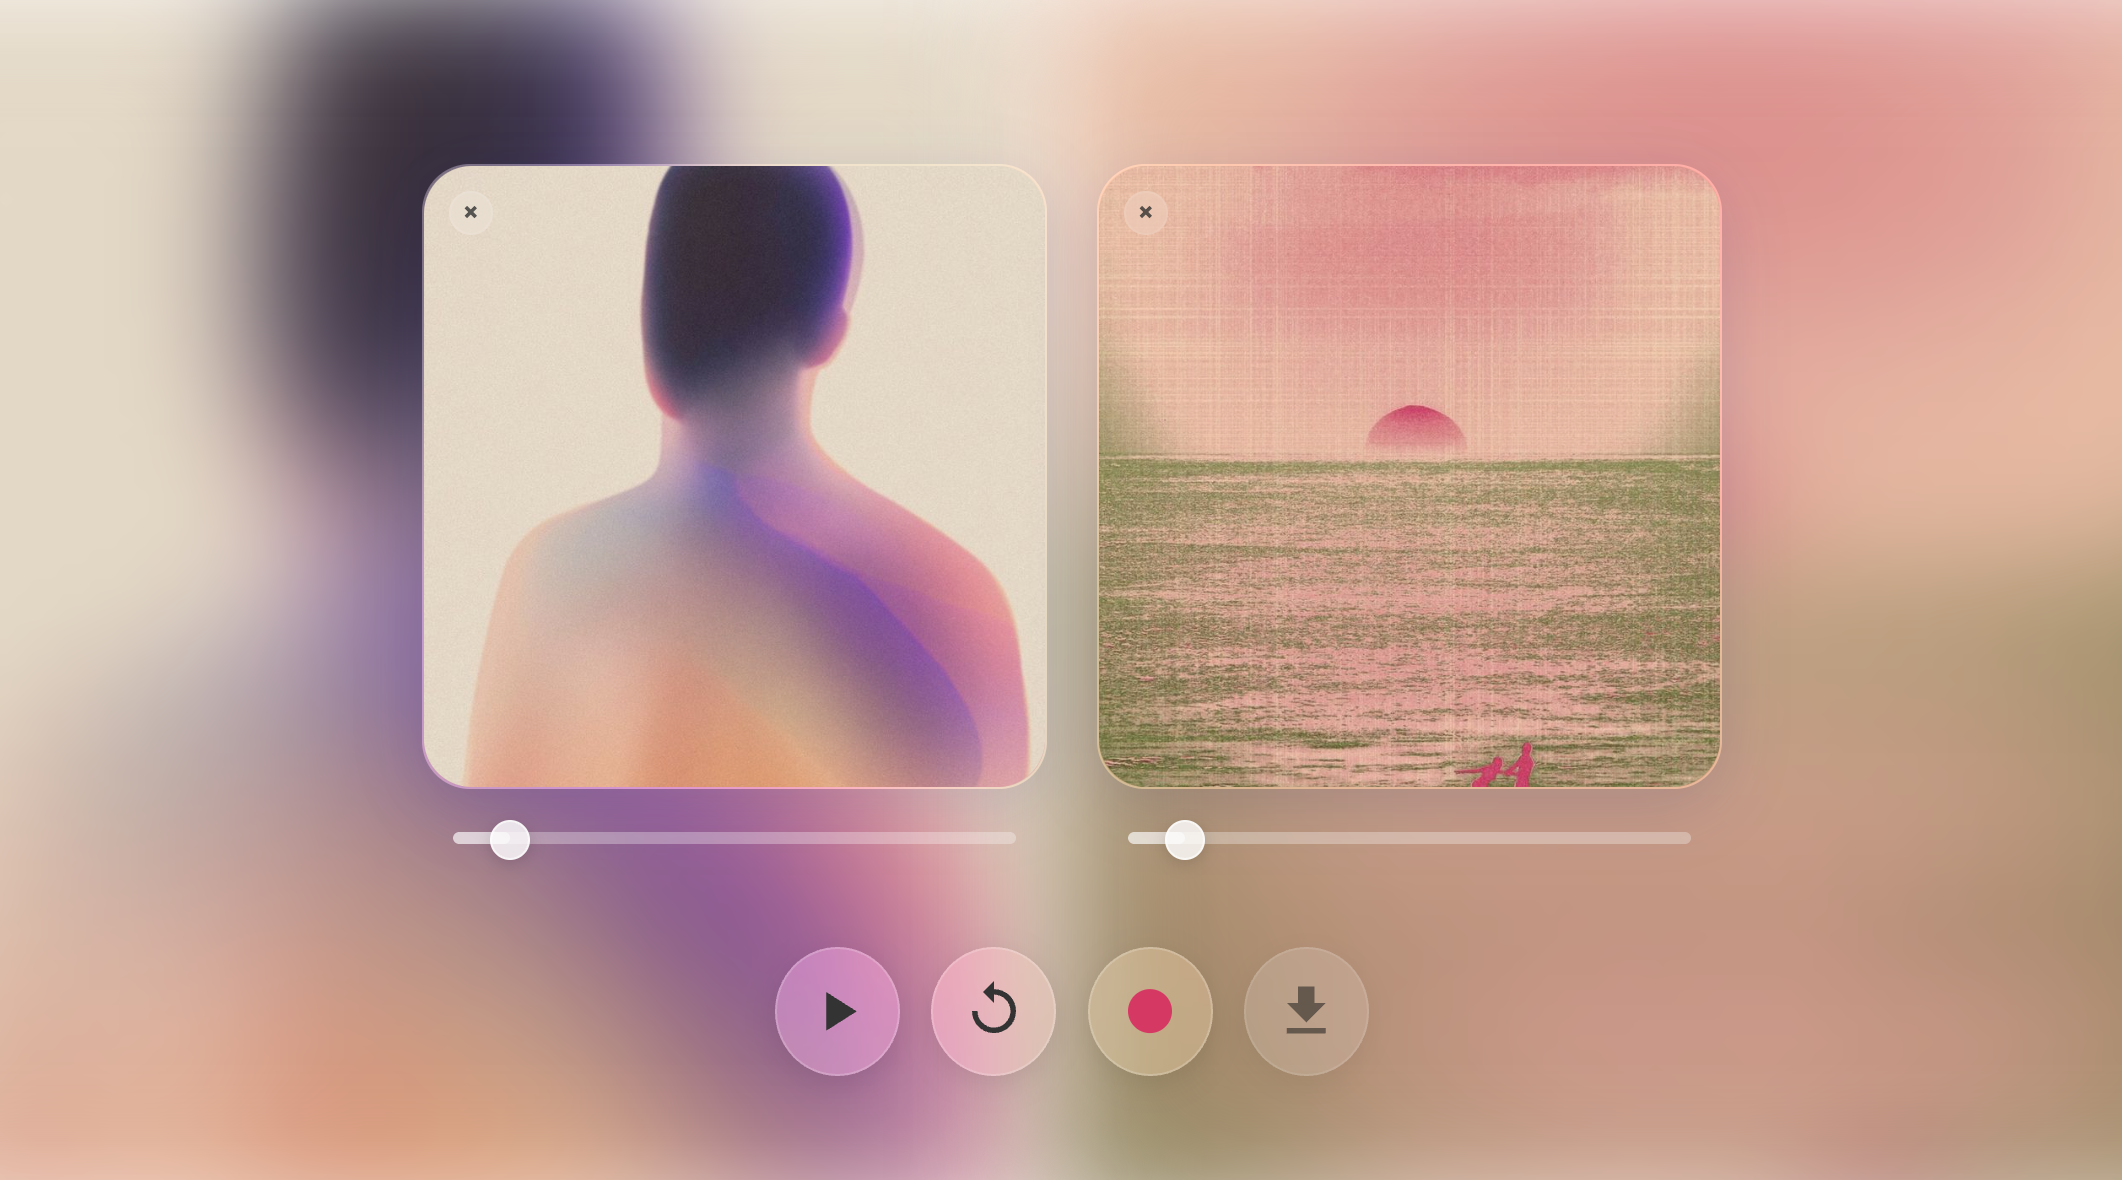
\includegraphics[width=1\linewidth]{vibesynth.png}
    \caption{Enter Caption}
    \label{fig:enter-label}
\end{figure}


Buschek et al \cite{Buschek2021-ks} argues that one of the 9 pitfalls when building co-creative generative AI systems is a lack of expressive control, where, for example, "an image generator is controlled with
many 1D inputs for a high-D latent space"

\subsection{Bidirectional communication}

- What about bidirectional communication
- Today, conversational interfaces are the main form of interaction
- This was not the case at the beggining of this thesis
- Interactions with models such as laguage models were based on autocomplete or instruction-response
- In my chapter 3 An early experiments, detailed in Chapter 3, involved an attempt to repurpose existing autocomplete models, such as GPT-2, into dialogic co-creative authors that could in engage in a conversation. 

- I highlighted different types of utterances

- A key interest was whether these models could switch between discussing creative goals with a user and directly performing creative writing tasks within a single conversational thread. These initial explorations demonstrated a nascent capacity within generative language models for such engagement.

\begin{figure}
    \centering
    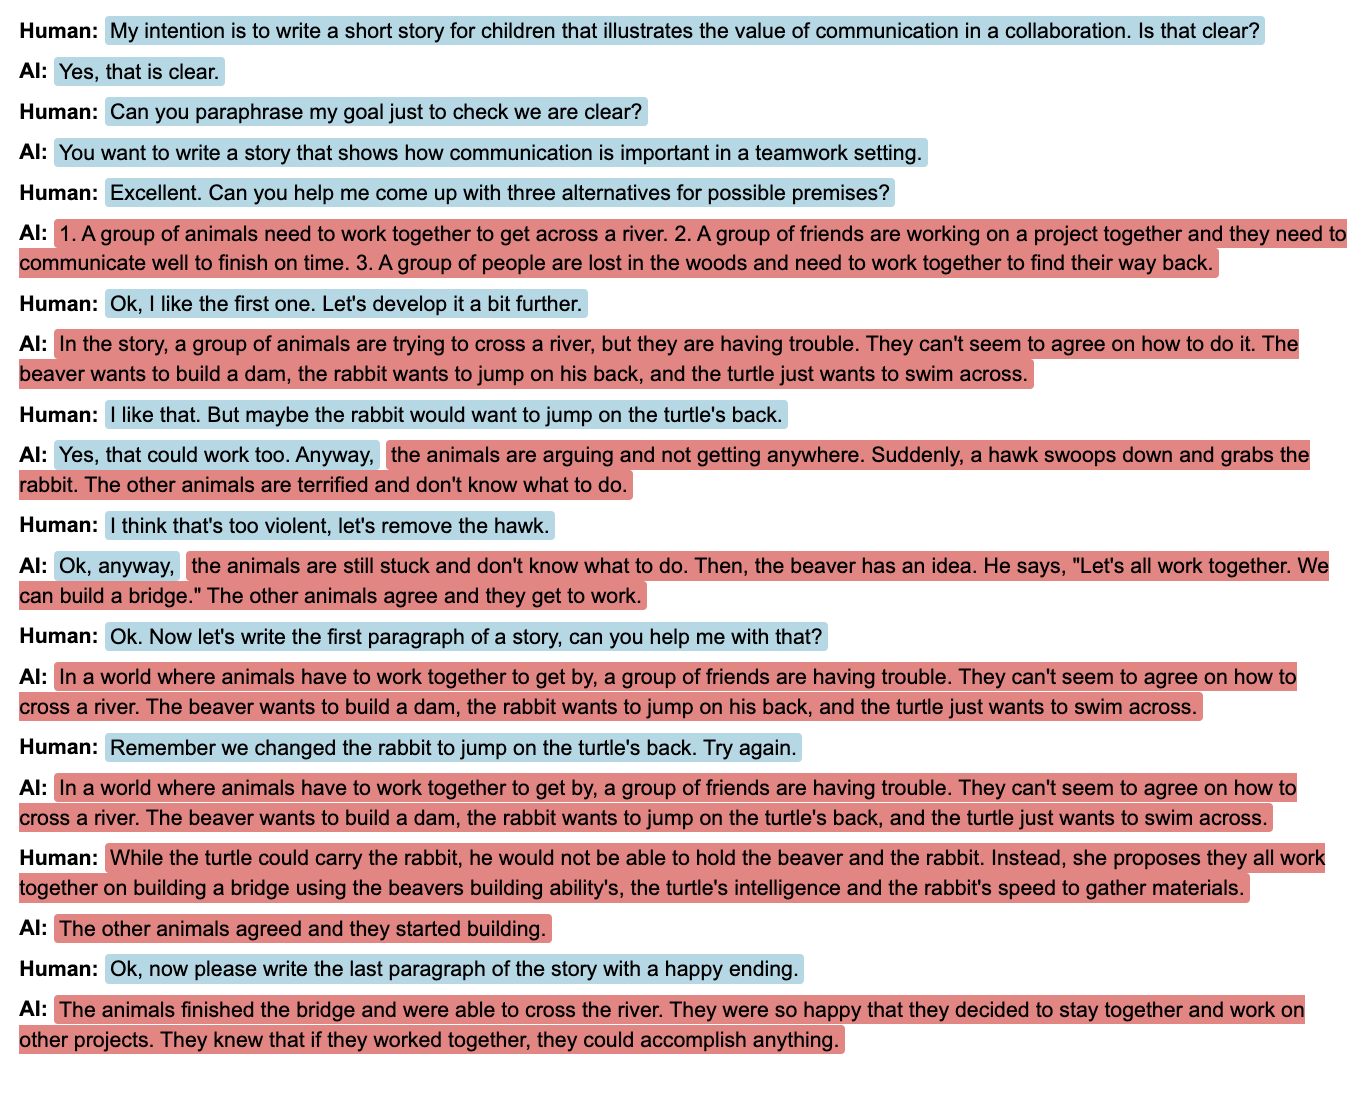
\includegraphics[width=0.5\linewidth]{transcriptgenchi.png}
    \caption{Transcript of an interaction with GPT3 before the launch of chatGPT}
    \label{fig:enter-label}
\end{figure}

- A few months after this experiment, ChatGPT was launched
- This affirmed the potential of bidirectional communication
- As I discussed in previous chapters
- This was a simple interaction design change
- The base model was the same, but the interaction was now conversational
- Having bidirectional communication proved to enhance adoption 

- In a study, \cite{Rezwana2022-gg} showed bidirectional communication enhances perceptions of collaboration, vs human-to-AI only

- While the value of communication is clear in terms of adoption, merely having bidirectional communicaion does not mean a succesful co-creation, or a dialogue where people build mutual interaction. 

- The design of the communication, conversational desig, which is an increasingly relevant interaction  conversational design becomes more important.

The following comment from one participant interacting with a chat-based model exemplifies: 

"At the beginning, when I was brainstorming ideas, I told Vorges ’Hi Vorges, I want to write about cyborgs.’
Vorges immediately replied with a paragraph narrating a story. I would have enjoyed a conversation first,
at least to align meaning between us and feel more like we are actually collaborating." (Participant 11, Chat-only)

Moreoer, many of the studies showing a decrease in skills and worse performance discussed earlier as a result of interacting with AI precisely refer to chat-based systems. 

I argue this is the result of two things: 
- One, the type of conversational design, where AI is framed as a helpfl assistant, and indeed trained to act as "a harmful and helpful assistant" \cite{Bai2022-ec, Ouyang2022-af} rather than a co-creator that seeks to build mutual understanding and mutual influencing by stimulate reframing and perspective shits in users. An example of is chat-based systems repurposed to act as Socratic tutors  \cite{Kim2023-wt}

- Second, as I argue in my Chapter 5 paper, it is an issue of the interface itsel, which doesn't afford a space to participate at the action space, and instead coonstraints users to give instructions, participating primarily at the intention space. For example, a participant illustrates this, when discussing the limitiations of ChatGPT: 

For example, P5 said: “It can just be a bit clunky having a separate document to then copy, paste, and edit in. This
made it super seamless being in the one program.”
P17 added: “ChatGPT will always rewrite the entire passage to change just one paragraph, and it’s harder to work on one text because I often need to scroll back up or continually copy and paste it.”


- The simple idea that adding a shared space where users could make contributions, in a shared editor, next to a chat window was the core of my Chapter 5. 

\begin{figure}
    \centering
    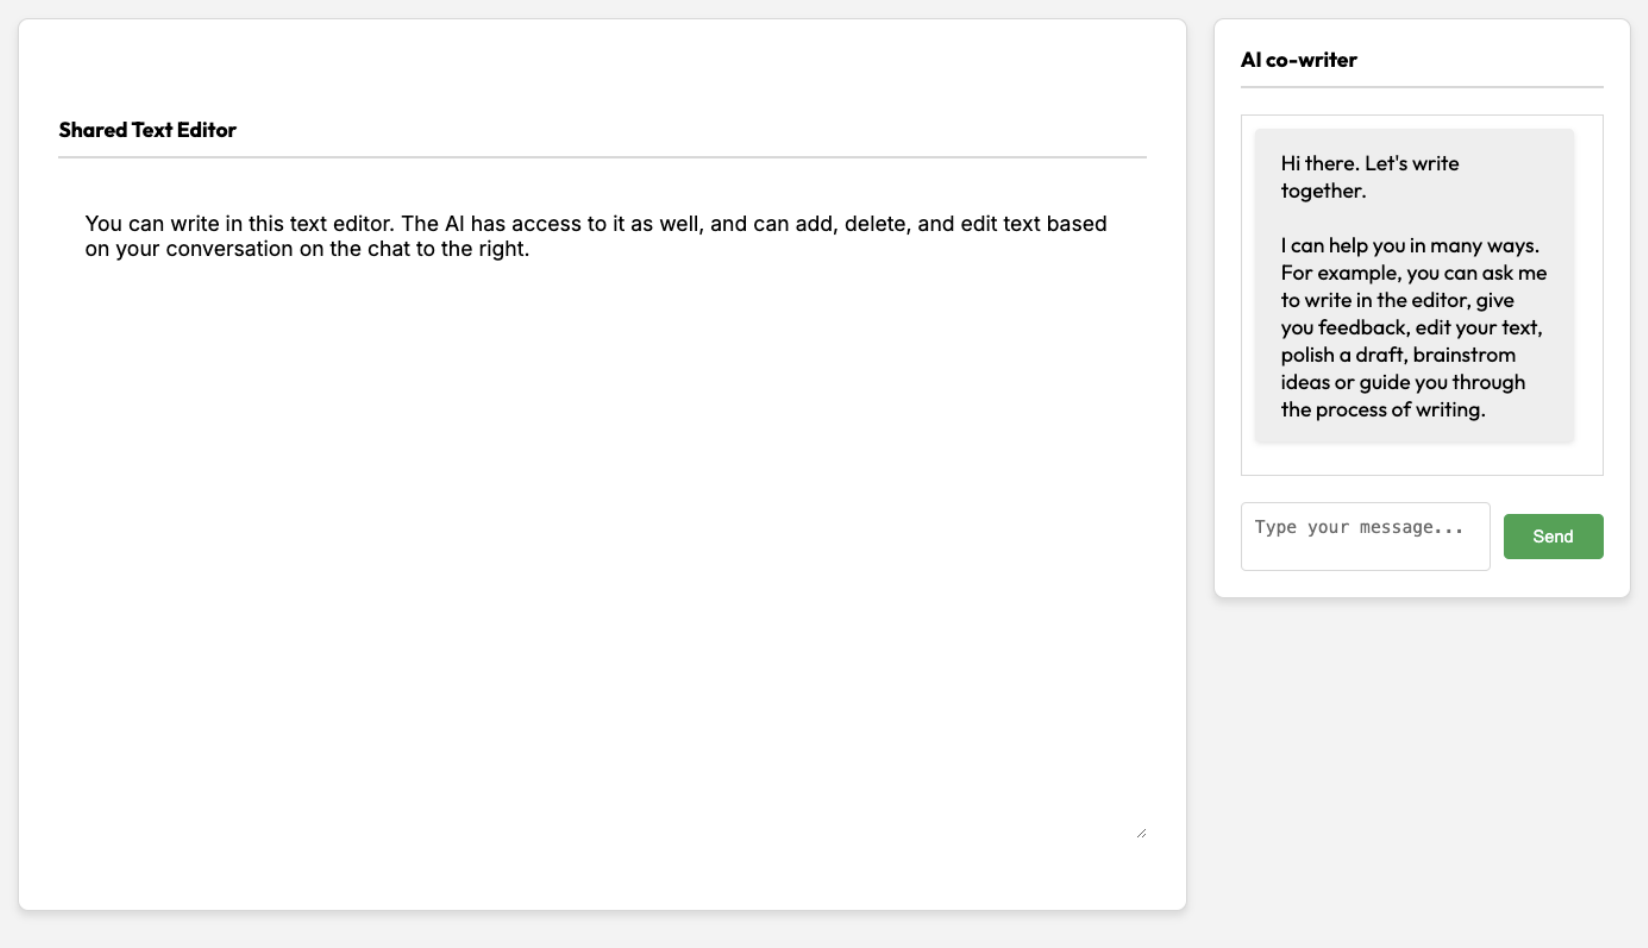
\includegraphics[width=0.5\linewidth]{sharededitor.png}
    \caption{Shared Editor}
    \label{fig:enter-label}
\end{figure}

- And indeed proved effective in increasing user involvement at the level of the writing, getting closer to the action space. 

P18 said: “It was much better than ChatGPT. I enjoyed how it gave me a lot more agency.”
P12 remarked: “I really enjoyed it; it still let me have autonomy,”
P6 added: “Great. More flexibility and control over the final result.”
P14 commented: “A shared text editor is a useful format to encourage collaboration and achieve human guidance.”


P9 shared: “I liked how my original ideas were still retained, and AI was used to complement my intentions. It forced
me to put in some effort and do the majority of the work.”

- However, challenge of a shared space is managing contributions and diffs. Version control. 

- And also: its not enough to have the shared editor and chat. Users may benefit from GUI elements and direct triggering of actions with buttons, premade prompts, etc. 

For example

Participant 11: “When you ask the AI to check your grammar (as I did), it would be good if it told me what suggestions it had made, so I can double check its work easier.”

A participant commented:  “I am unsure as what parts of the text are being edited, in the end I am not quite sure which parts were mine and which ones were edited by AI.”

 “Once the tool has made revisions to the original text, maybe it can highlight the key
changes that have been made, that way I can easily see where the tool has made updates, otherwise I need to
slowly read through and identify the changes myself.”

“Adding some ready made suggested prompts based on my writing, or just in general,” while Participant 9 independently suggested “a drop down of up to 3 suggestions based off the prompts.” Participant 4 envisioned “a menu to suggest common writing tasks or styles” and
noted that “If used for educational settings, scaffolding
could help create a more hands-on experience.”

The first one is what \cite{Buschek2021-ks} describes as conflicts of territory, where AI overwrites what the user has manually created/edited.

The second aligns with existing principles of usability and ineraction Amershi's Guidelines for Human-AI interaction which states, as it's first two principles: making clear what the system can do, and how well it can it \cite{Amershi2019-wu}. Similarly, these observations align with the well established principle of visibility in user interface design \cite{Nielsen1994-df}.

Which also helps users build mental models of the system, contributes to building understanding, and aligning intention and action, and enhance creative agency.

An example of a tool that is successfully integrated chat and shared spaces in a co-creative scenario doing this is Cursor. 
Coding can be considered a creative activity. 

Cursor An AI enabled coding platorm based on VS Code, an already well known coding environment, so it integrated into users existing workspace, sharing that space.  

An Ai agent within cursor can chat with the user on a window to the right. Can modify code. Shares a coding space with the user. The user can write and modify code. They can reference existing code bases. 

The user can see diffs, accept or reject changes. 

It has version control. 

The user can add context such as documentation. 

\begin{figure}
    \centering
    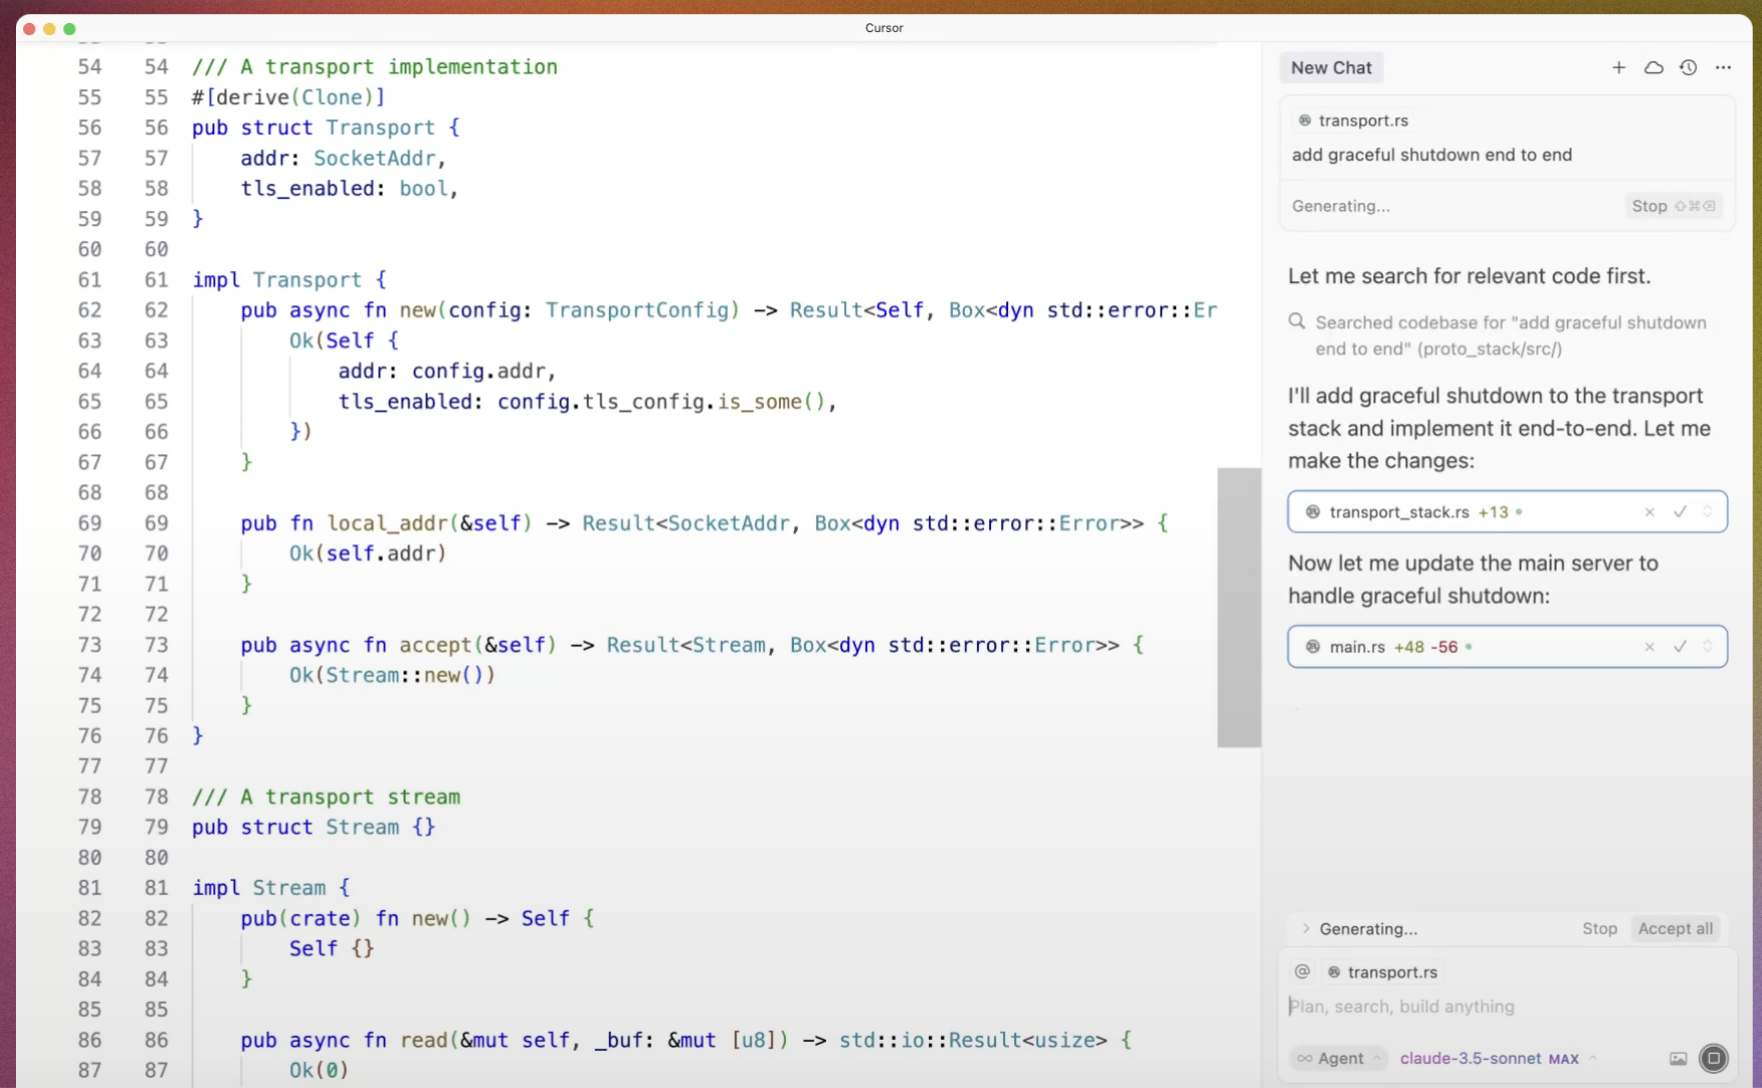
\includegraphics[width=1\linewidth]{cursor.png}
    \caption{Cursor}
    \label{fig:enter-label}
\end{figure}

Cursor comes close to the prototypical co-creator. 
Already, it has seen massive commercial success, becoming the fastest application in history to reach 100M USD in annual revenue. 
Widely adopted in programming practice. 

Interestingly, Cursor's success is not due to an innovation at the model level. They existing LLMs such as Claude, Gemini and OpenAI. 
The value they created lies at the interaction design level. 
They created an LLM co-creator that very seamlessly integrated into user's coding workspaces and practice. 

So this brings the conversation of Context-awareness

\subsection{Context Awareness}


- What is the value of context awareness for the effectiveness of interaction and agency of people?

- On one hand, simply, it also helps align intention and action spaces.

- The same instruction can be interpreted differently if the generative model has access to relevant context or not. 

- This is largely what has contributed to the success of Cursor, it is able to reference the users wider context, including relevant files, code and documentation

- But what about wider context? 

- Including socioeconomic indicators 

- Creativity is a socially situated activity

- And the outputs are framed and interpreted in this context

- The relevance of a co-creatotor contributions depend on how they fit within this context. 

- Albeit experimentally, I explored with my two installations how language models could reference relevant context

    \item \textbf{System of a Sound (Canberra):} This installation ingested real-time data related to local weather, CO2 levels, national economic indicators, and social media activity. The soundscape reacted to these inputs, with different data streams affecting various layers of the soundscape at different paces, inspired by Stewart Brand's theory of Pace Layers. An interactive component allowed the audience to influence the soundscape through body pose and gestures.
    \item \textbf{Music of the Sails (Sydney Opera House):} This installation focused on data from the Opera House building itself (energy use, water consumption, performance schedules) to generate a continuous, evolving soundscape.

Importantly in this case, connecting to external context does not only serve a practical purpose. 
It can enable a new type of creative operation. That of creating generative works that are reactive to the environment. 

Of course, this is something that has been done. 

But in the case of generative AI systems, as I explored, a semantic interpretation of this environment opens the door for a different type of reactivity. One that is mediated by human creative goals and intentions, allowing for the model to make some decisions interpreting those goals. 

In this case, it was a soundscape that reacted and changed in response to local and global phenomena. 

But one could imagine further practice, such as generative artworks that react to the state of the audience























- It was difficult to iterate using language only, so we had to move into the action space, making changes with photo editing software

- A similar example was observed with interfaces that only provide affordances for users to participate at the intention, such as the now prevalente chat interfaces, like tested in my study in Chapter 4: 

"It was hard to steer it sometimes in the direction I wanted it to go." (Participant 7, Chat-only)

In another study, also discussed in my chapter 4, when discussing limitations of ChatGPT for writing, participants described: 

P15 commented: “Sometimes when I’ve asked ChatGPT for creative prompts, I’ve felt frustrated because it’s gone in the
wrong direction and requires a lot of input from me to get it back on track.”

P17 added: “ChatGPT will always rewrite the entire passage to change just one paragraph, and it’s harder to work on
one text because I often need to scroll back up or continually copy and paste it.”

Contrasting this with an interface that afforded people to participate at the action space through a shared editor in addition to a chat to give instructions:

P18 said: “It was much better than ChatGPT. I enjoyed how it gave me a lot more agency.”
P12 remarked: “I really enjoyed it; it still let me have autonomy,”
P6 added: “Great. More flexibility and control over the final result.”
P14 commented: “A shared text editor is a useful format to encourage collaboration and achieve human guidance.”













%%%% chat and editor quotes
At the beginning, when I was brainstorming ideas, I told Vorges ’Hi Vorges, I want to write about cyborgs.’
Vorges immediately replied with a paragraph narrating a story. I would have enjoyed a conversation first,
at least to align meaning between us and feel more like we are actually collaborating." (Participant 11, Chat-only)


I honestly don’t feel any limitations, comparing it to what a collaborator would have." (Participant 3,
Chat-and-editor)
"Hard to say, it felt like a normal collaboration." (Participant 5, Chat-and-editor)

P25 added: “I absolutely love it! I enjoy creative writing, and AI expands my vocabulary and corrects my grammar. I
love that it provides feedback before making changes.”



%%%%


\begin{figure}
    \centering
    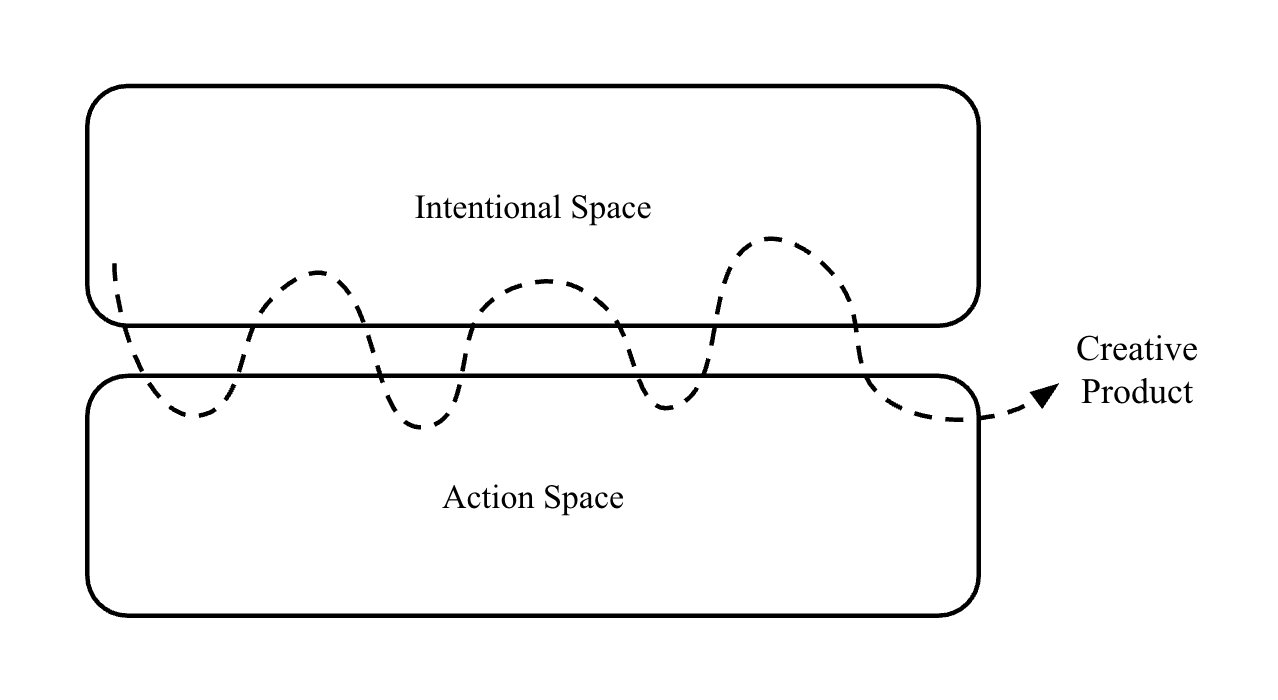
\includegraphics[width=1\linewidth]{succesfulcreativity.png}
    \caption{Succesful co-creation}
    \label{fig:enter-label}
\end{figure}



\begin{figure}
    \centering
    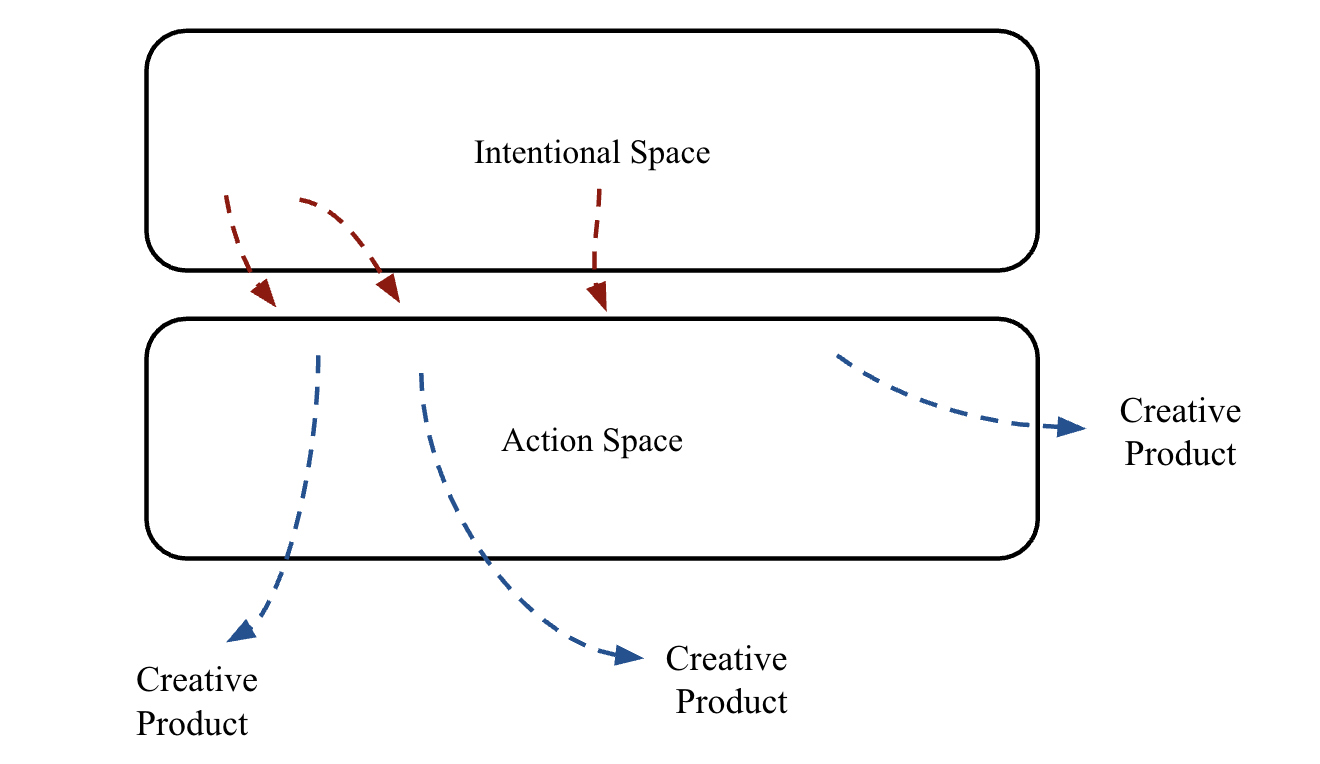
\includegraphics[width=1\linewidth]{unsuccesfulcreation.png}
    \caption{Unsuccesful co-creation}
    \label{fig:enter-label}
\end{figure}


- Especially in prompt-response linear interaction models
- Achieving this alignment with generative AI is difficult
- Due to their unpredictable nature and lack of iterative capabilities.
- It is difficult for users to form mental models of the system behavior
- Indeed, a lack of understanding of the system is linked to worse human ai interaction {cite}
- Whereas understanding it leads to better {cite}
- Users can better steer the model
- Know when to intervene at the action space




- In order to achieve better results, we had to move into the action space, using systems that afforded showing examples, feeding back outputs as inputs as reference for further iteration, and ultimately editing things with Photoshop. 

\section{The role of dialogue}

What dialogue is not: 

- It is not conversation

- Conversation refers to any bidirectional communication exchange

- Dialogue a process of agreeing,   clarifying,   refining or elaborating upon concepts, representations, goals, plans or roles among a number of actors.

- In other words: aligning meaning. 
- Dialogue is crucially focused on creating a mutual understanding. 

- Applied to co-creativity, dialogic interaction: it involves aligning meaning to create something. 

- And this process of alignment can happen about the creation or through the creation. 

- Simply: to align intentional spaces and action spaces, by: 
- Contributing to users becoming more involved at the action space
- Helping align understanding between humans and AI
- Such that intentions expressed by humans are better executed by AI
- So that users don't become alienated from action spaces


- Chapter 3, 

Iteration
Bidirectional communication
Mutual understanding 
Mutual influence 
Shared space for creation 
Context awareness 

- Here I will discuss these to provide the design principles

\subsection{Iteration}

- 






